\documentclass{article}%
\usepackage[T1]{fontenc}%
\usepackage[utf8]{inputenc}%
\usepackage{lmodern}%
\usepackage{textcomp}%
\usepackage{lastpage}%
\usepackage{geometry}%
\geometry{hmargin=1cm,vmargin=2cm,paper=a4paper}%
\usepackage{ragged2e}%
\usepackage{amsmath}%
\usepackage{graphicx}%
\usepackage{fancyhdr}%
%
\fancypagestyle{header}{%
\renewcommand{\headrulewidth}{0pt}%
\renewcommand{\footrulewidth}{0pt}%
\fancyhead{%
}%
\fancyfoot{%
}%
\fancyhead[L]{%
Date: %
\linebreak%
2026{-}08{-}19%
}%
\fancyhead[R]{%
Whale Watch Workhorse%
}%
\fancyfoot[C]{%
Page \thepage\ of \pageref{LastPage}%
}%
}%
%
\begin{document}%
\normalsize%
\pagestyle{header}%
\begin{minipage}{\textwidth}%
\centering%
\begin{Large}%
\textbf{Underwater Noise Impact Assessment}%
\end{Large}%
\linebreak%
\linebreak%
\begin{large}%
\textbf{Sound source: Sercel Micro{-}GI Air Gun}%
\end{large}%
\linebreak%
\begin{large}%
\textbf{Animal group: VHF}%
\end{large}%
\end{minipage}%
\section{General information}%
\label{sec:Generalinformation}%
\subsection{Animal group VHF}%
\label{subsec:AnimalgroupVHF}%
Very High{-}frequency (VHF) Cetaceans including Delphinidae (Cephalorhynchus spp.; Lagenorhynchus cruciger, L. austrailis); Phocoenidae (Neophocaena spp., Phocoena spp., Phocoenoides); Iniidae (Inia); Kogiidae (Kogia); Lipotidae (Lipotes); Pontoporiidae (Pontoporia)\newline%
%
\linebreak%
Permanent and Temporary Threshold Shift (PTS, TTS) limits are determined                         with the more conservative measure of the dual exposure metrics                       of unweighted zero{-}peak Sound Pressure Level as compiled from                      Southall et al. (2007, 2019); BOEM (2014a,b); Statoil ASA (2015);                       Tougaard et al. (2014, 2015, 2016); Schack et al. (2019): %
\begin{alignat*}{2}%
SPL_{uw,0-peak}(PTS) &=%
202%
\,dB\,re\,1\,\mu\,Pa%
\end{alignat*}%
\begin{alignat*}{2}%
SPL_{uw,0-peak}(TTS) &=%
196%
\,dB\,re\,1\,\mu\,Pa%
\end{alignat*}%
 and the weighted Sound Exposure Level:%
\begin{alignat*}{2}%
SEL_{w}(PTS) &=%
155%
\,dB\,re\,1\,\mu\,Pa^2 s%
\end{alignat*}%
\begin{alignat*}{2}%
SEL_{w}(TTS) &=%
140%
\,dB\,re\,1\,\mu\,Pa^2 s%
\end{alignat*}%
The noise limits for behavioral effects are based on the weighted Root                         Mean Square Sound Pressure Level with an averaging time of 125 ms (Tougaard et al., 2014, 2015, 2016):%
\begin{alignat*}{2}%
SPL_{w,rms} &=%
103%
\,dB\,re\,1\,\mu\,Pa%
\end{alignat*}%
\newpage

%
\subsection{Sound Source Sercel Micro{-}GI Air Gun}%
\label{subsec:SoundSourceSercelMicro{-}GIAirGun}%
The source wavelet is shown in the upper panel of                         Figure 1. In the second the source spectrum is given.                         This is contrasted with the hearing threshold of the VHF in the third panel. The signal is characterized by a frequency content of 1.3e+02 Hz to 4.8e+02 Hz at {-}6 dB relative to the maximum power, a pulse length of 4.0 ms and the following UNweighted                         source intensities at a reference distance of 1m:%
\begin{alignat*}{2}%
SPL_{uw,0-peak}(1\,m) &=%
226.0%
\,dB\,re\,1\,\mu\,Pa%
\end{alignat*}%
\begin{alignat*}{2}%
SEL_{uw}(1\,m) &=%
196.0%
\,dB\,re\,1\,\mu\,Pa^2 s%
\end{alignat*}%


\begin{figure}[h!]%
\centering%
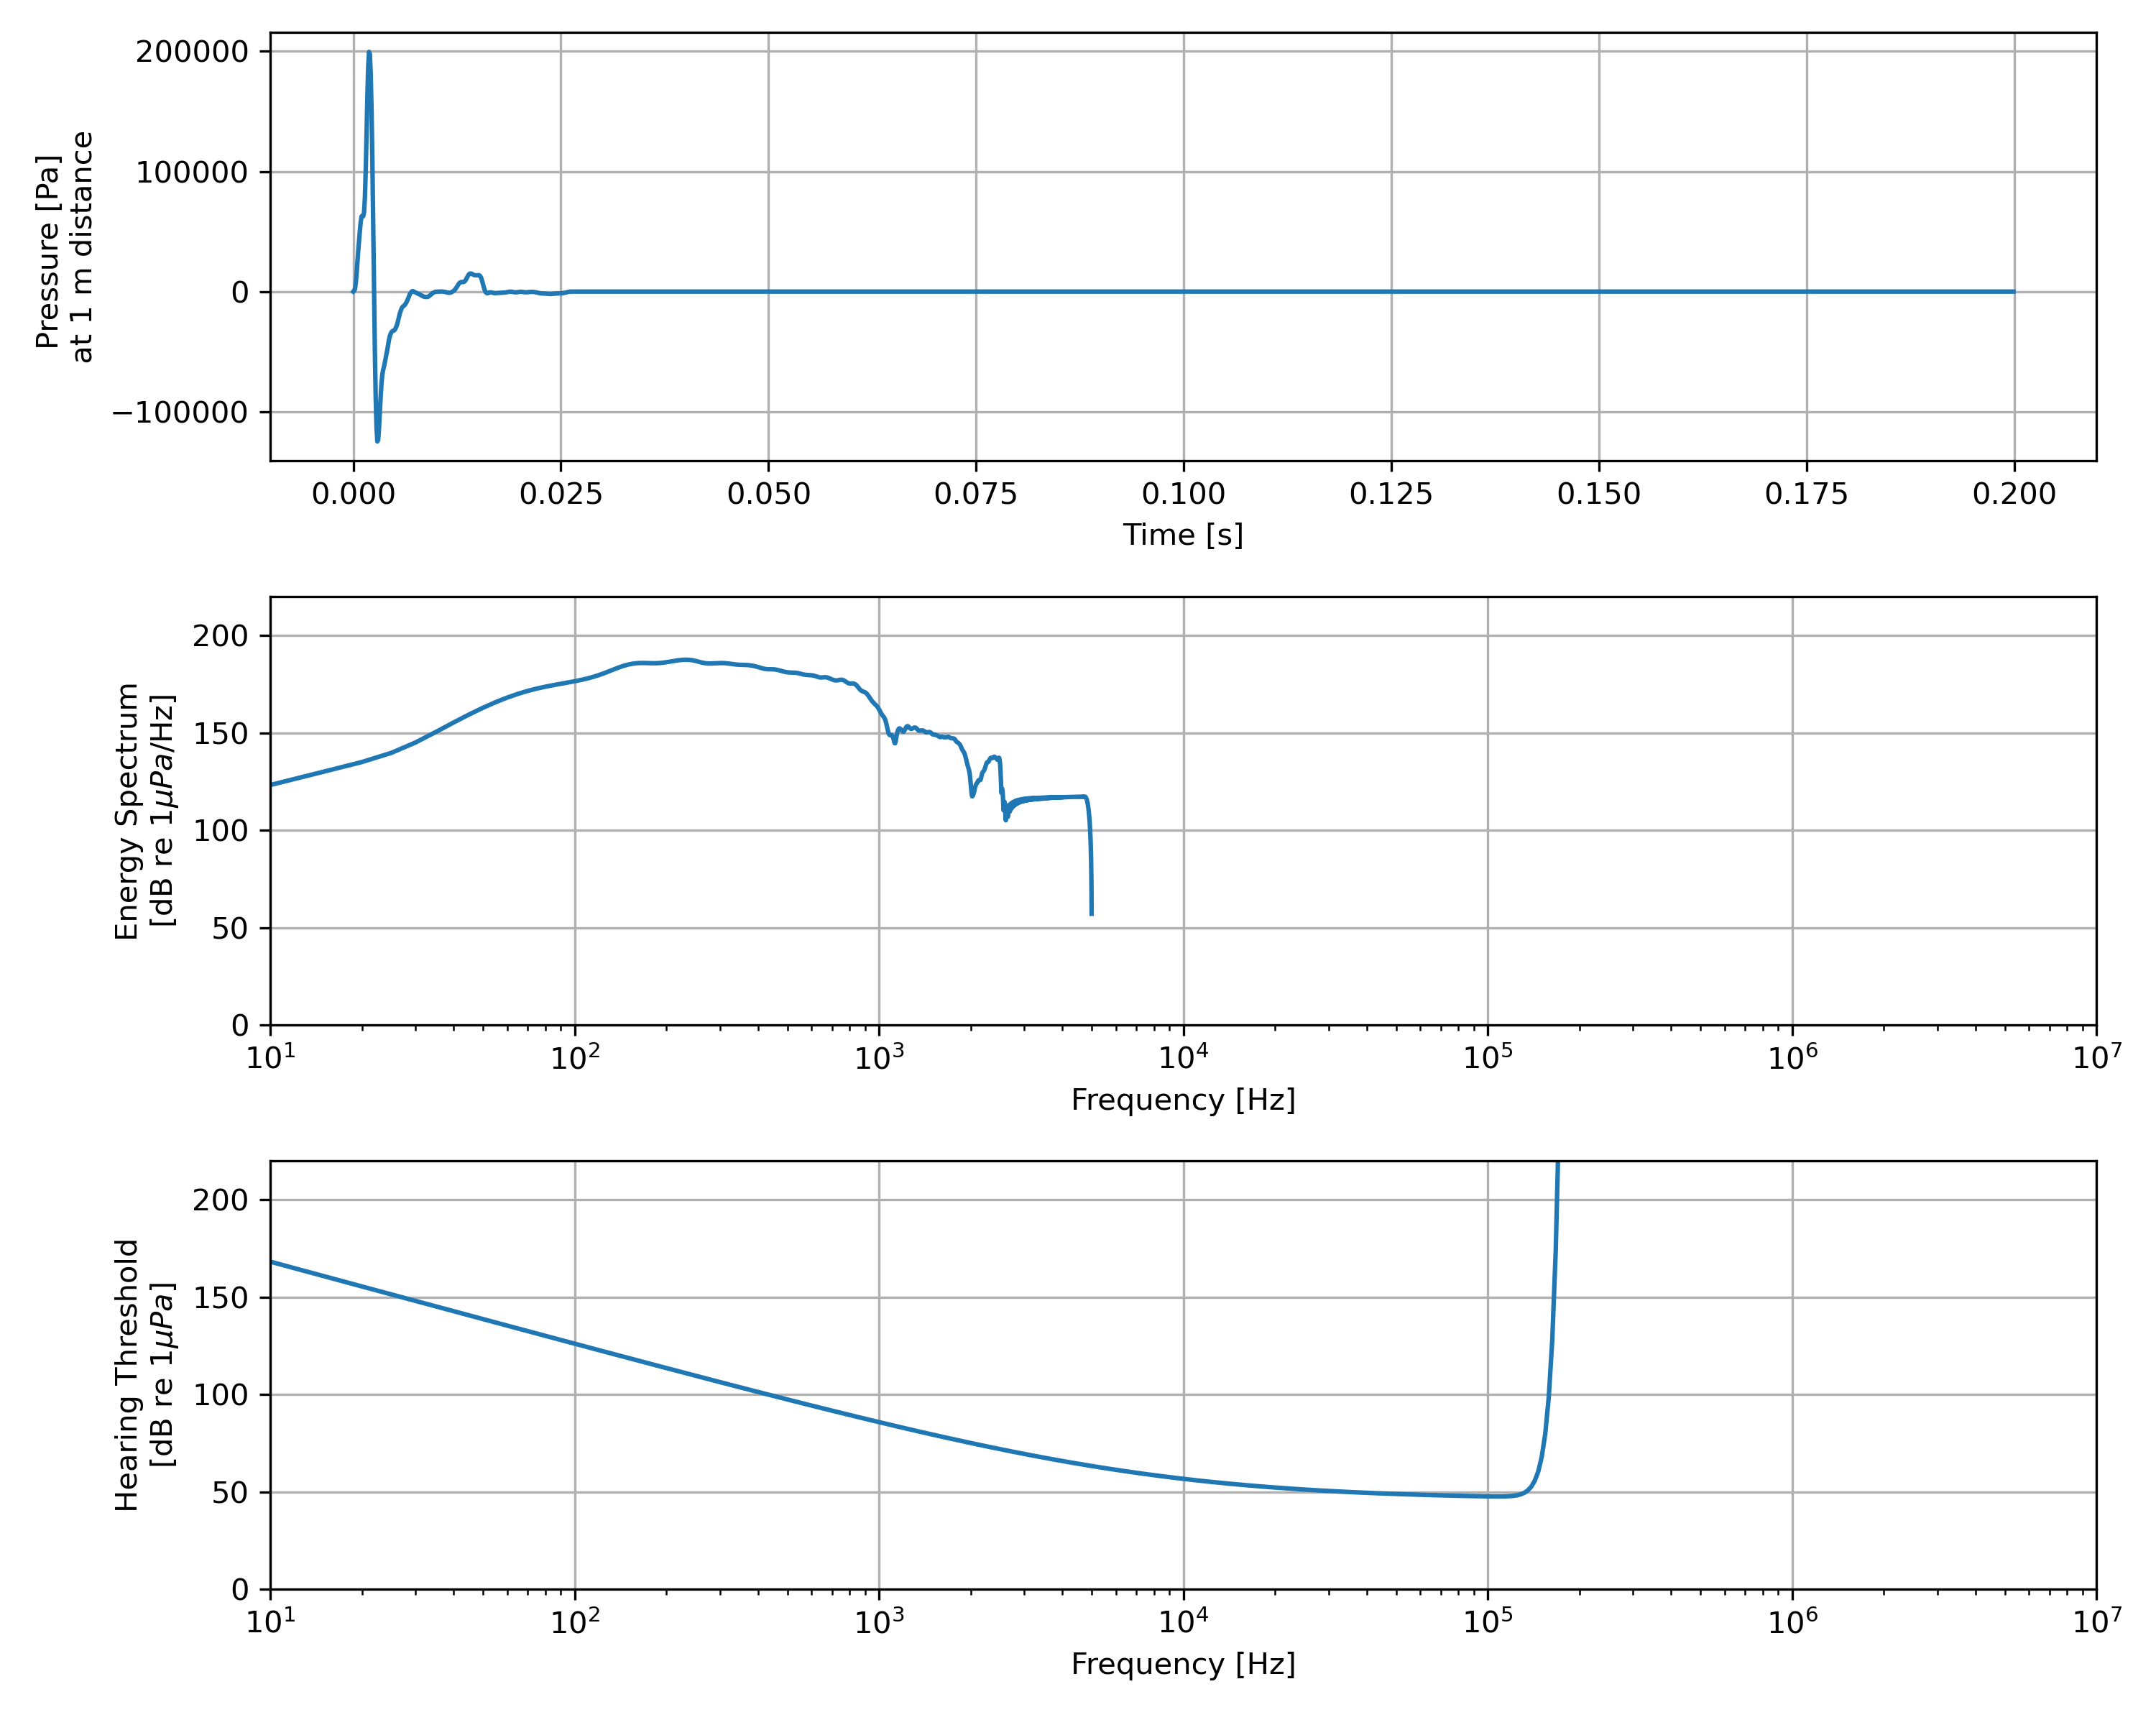
\includegraphics[width=300pt]{Seismics_Source}%
\caption{Source characteristics of the Sercel Micro{-}GI Air Gun; First panel: Time series of the wavelet record;                     Second panel: Source power spectrum; Third panel: Hearing threshold of the VHF.}%
\end{figure}

%
For a single seismic source, the directivity is estimated                         with the Lloyds Mirror effect based on Carey (2009).                         The most relevant factors are the dominant frequency of 440.0 Hz and the source tow depth of 0.7 m. The resulting and applied directivity                         are shown in Figure 2.%


\begin{figure}[h!]%
\centering%
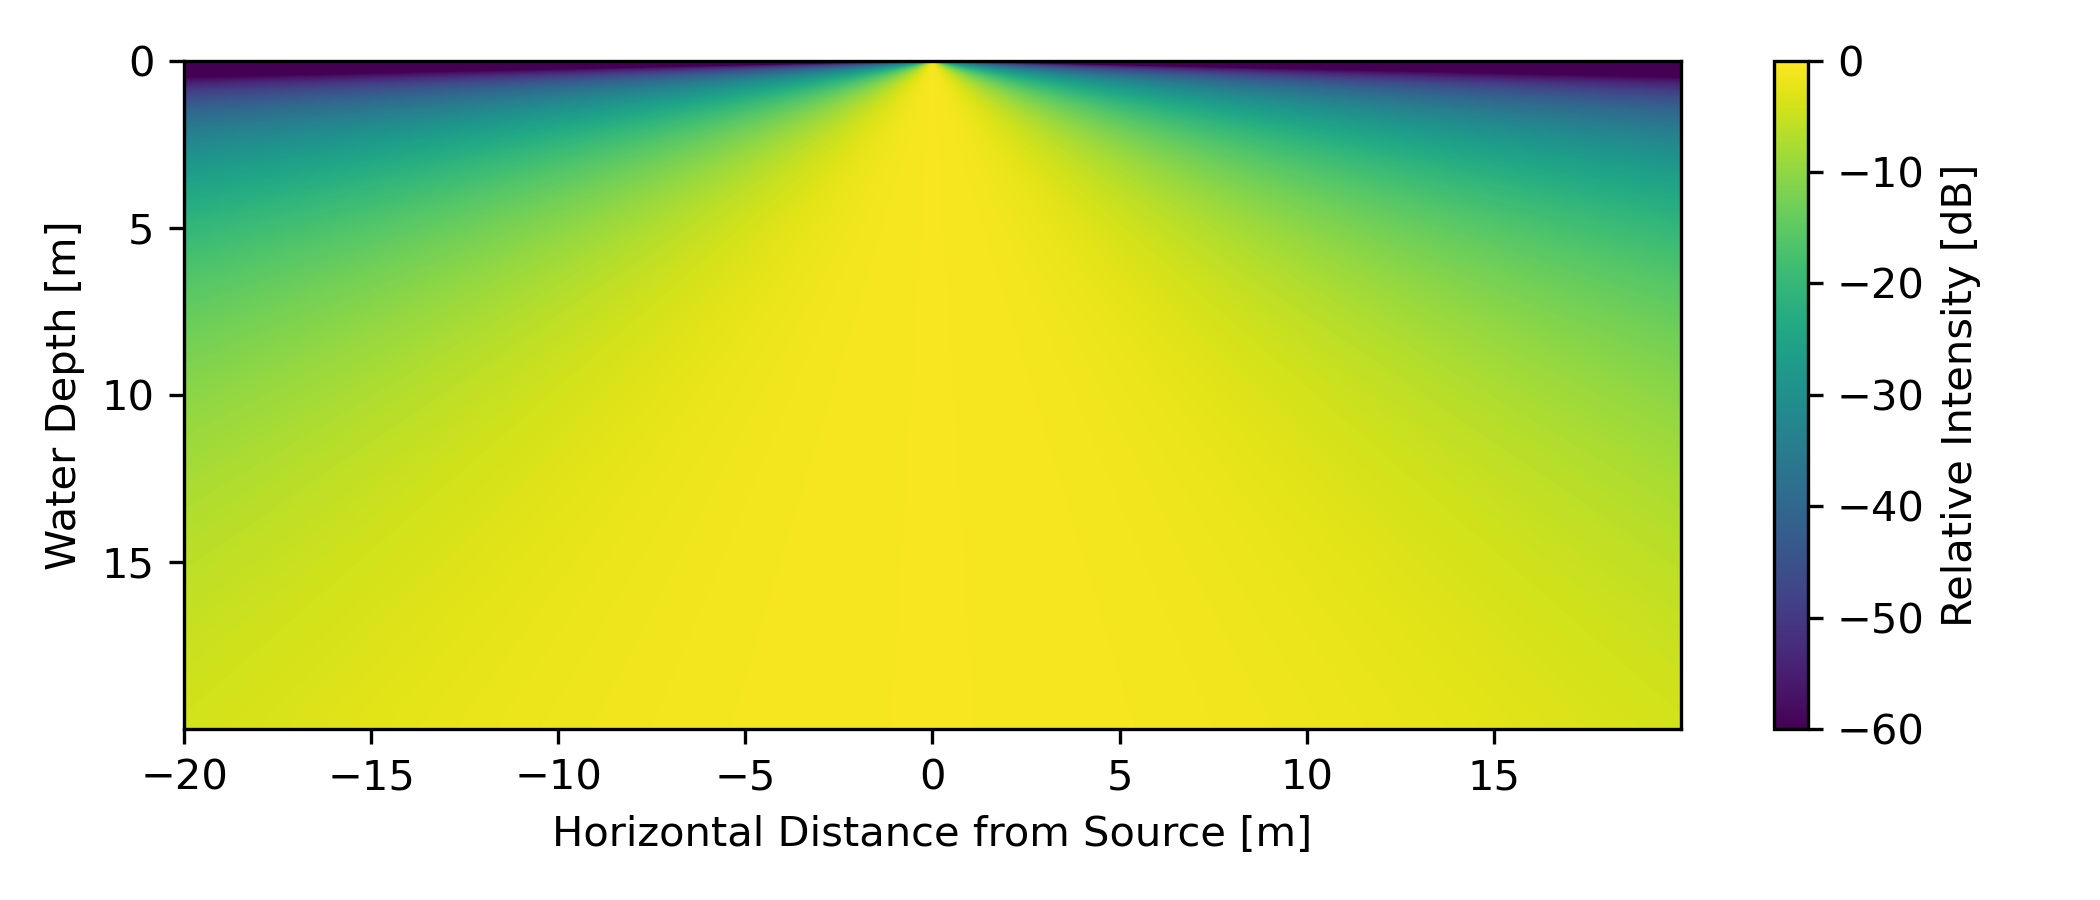
\includegraphics[width=300pt]{Seismics_Source_Directivity}%
\end{figure}

%


\begin{figure}[h!]%
\centering%
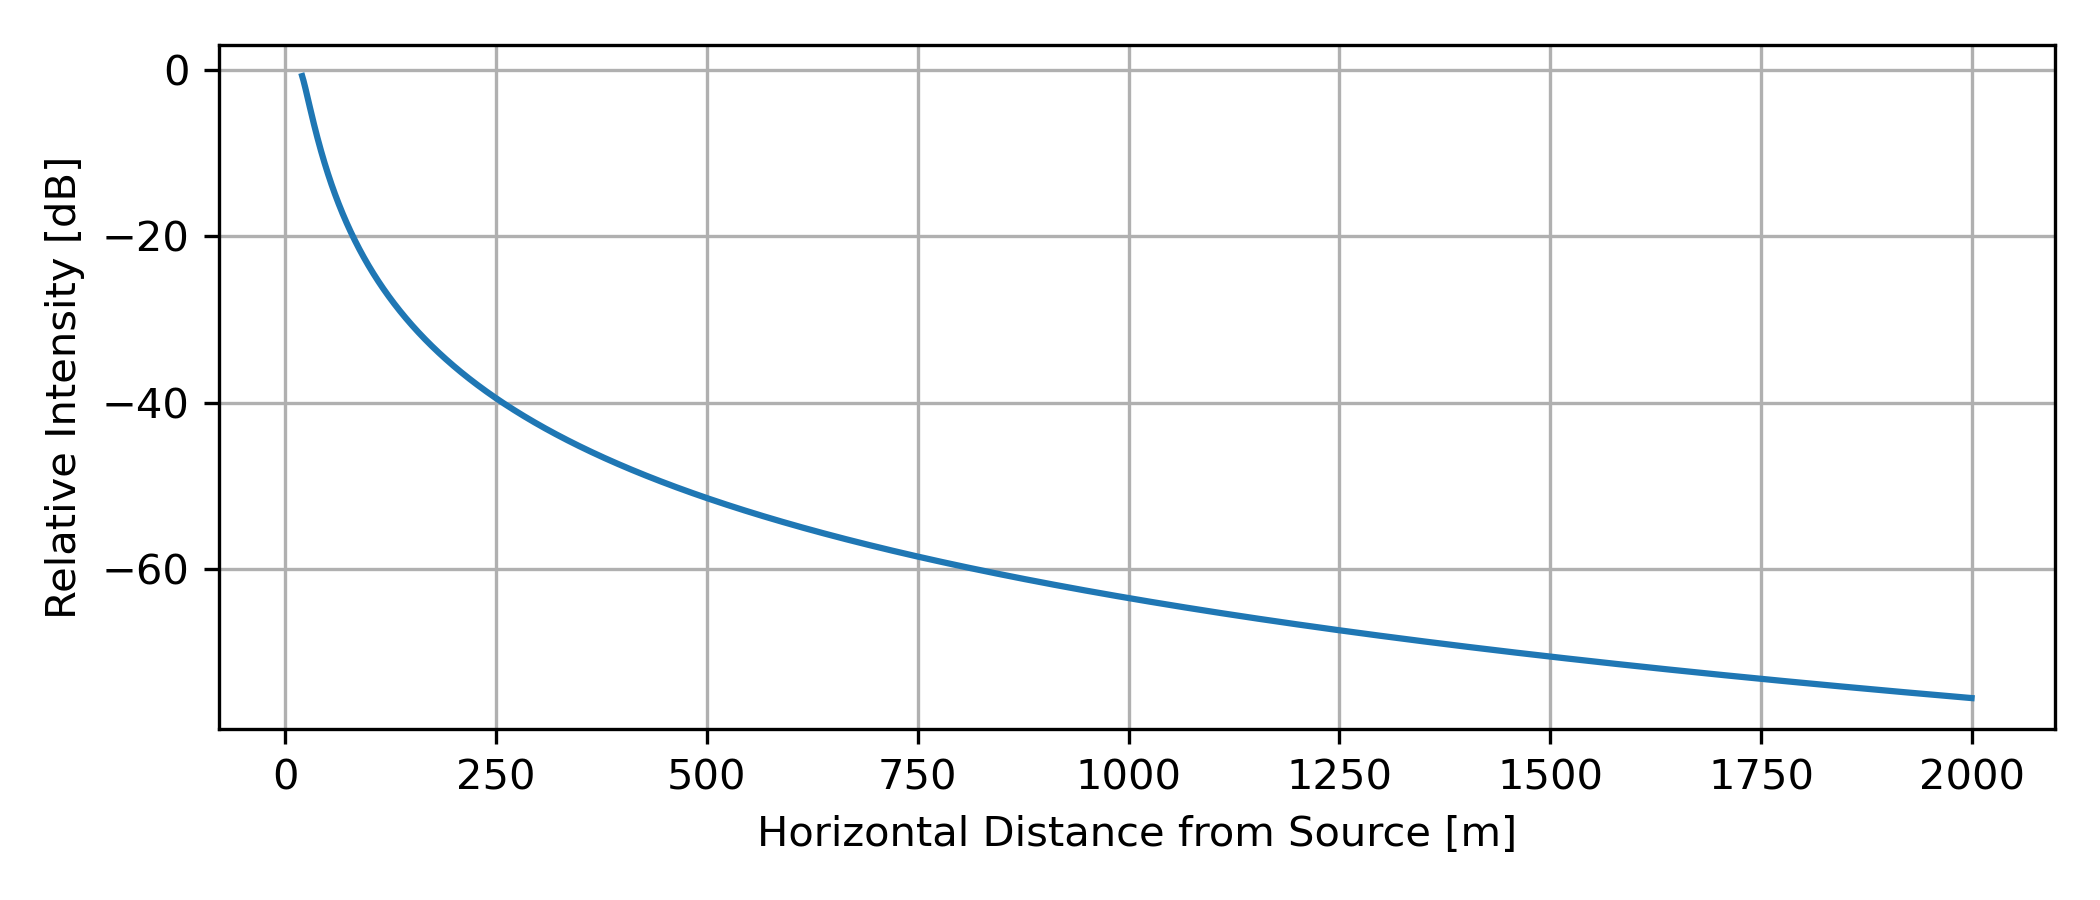
\includegraphics[width=300pt]{Seismics_Source_DirectivityApply}%
\caption{Upper panel: Calculated directivity,                     Lower panel: Directivity function applied to the exposure metric calculation.}%
\end{figure}

%
\newpage

%
\section{Calculation Basics}%
\label{sec:CalculationBasics}%
For the calculation of the metrics, knowledge about the                     geometric spreading as shwon in Figure 2, absorption and the filter function                     for the functional hearing group are relevant.%
\subsection{Geometric Spreading}%
\label{subsec:GeometricSpreading}%
To account for the geometric spreading, the ShallowWater{-}model is used               (see e.g. Elmer et al., 2007; Bradley and Stern, 2008; Duncan and Parsons, 2011). For this geometric spreading model, the waterdepth 20 m and the safety threshold {-}6.6 dB are relevant.%


\begin{figure}[h!]%
\centering%
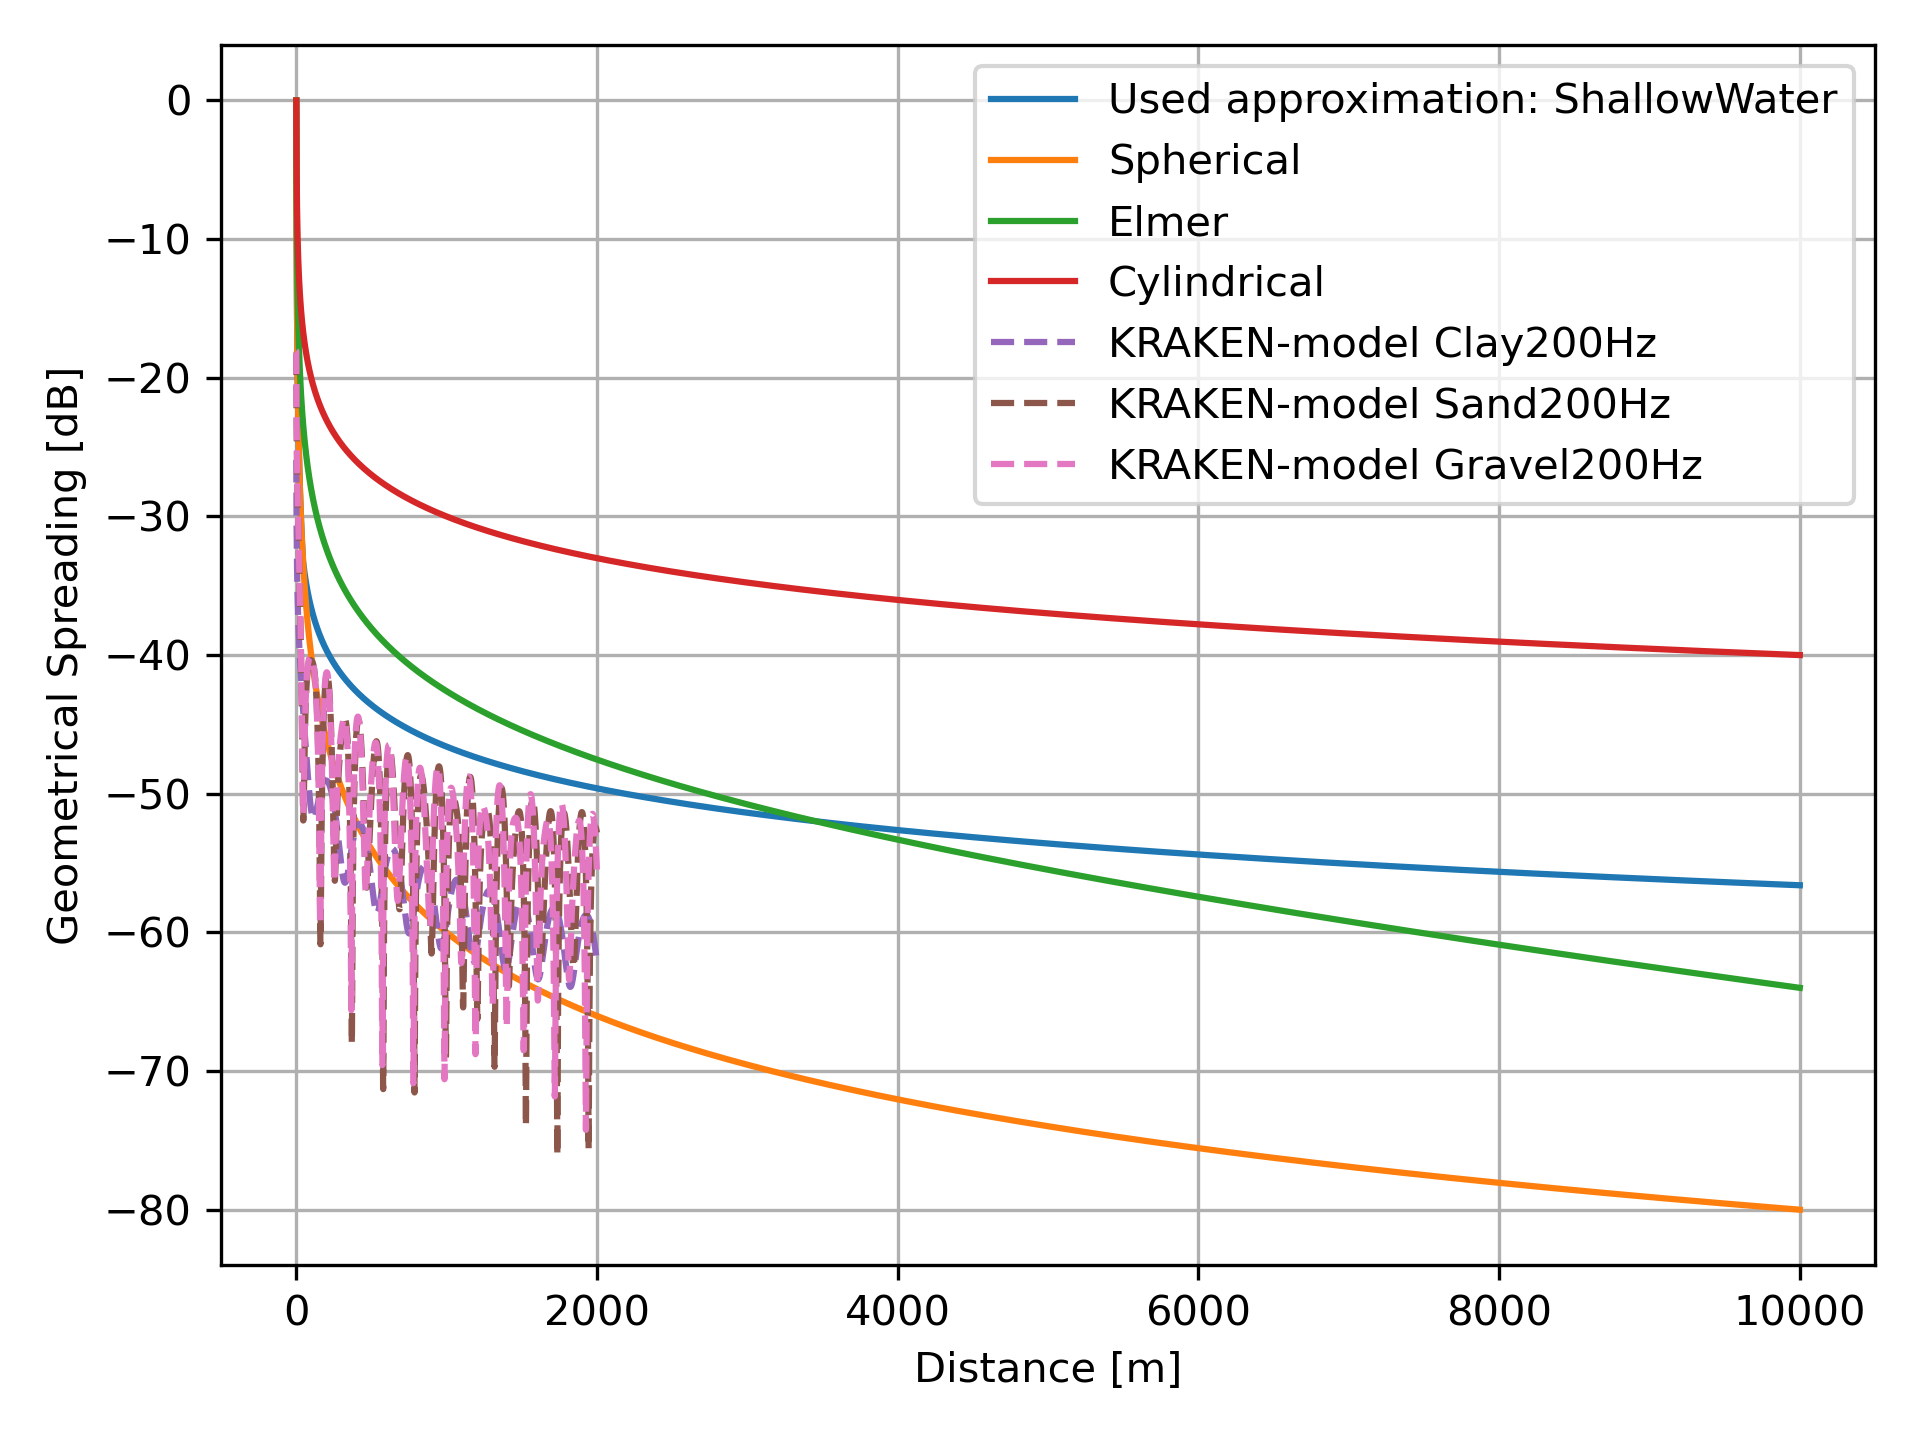
\includegraphics[width=300pt]{Seismics_Spreading}%
\caption{Geometric spreading approximations;                     The used approximation is drawn as a blue solid line.}%
\end{figure}

%
\subsection{Absorption}%
\label{subsec:Absorption}%
The absorption is calculated according to Ainslie and McColm (1998)                        for the Baltic Sea and shwon in Figure 3.%


\begin{figure}[h!]%
\centering%
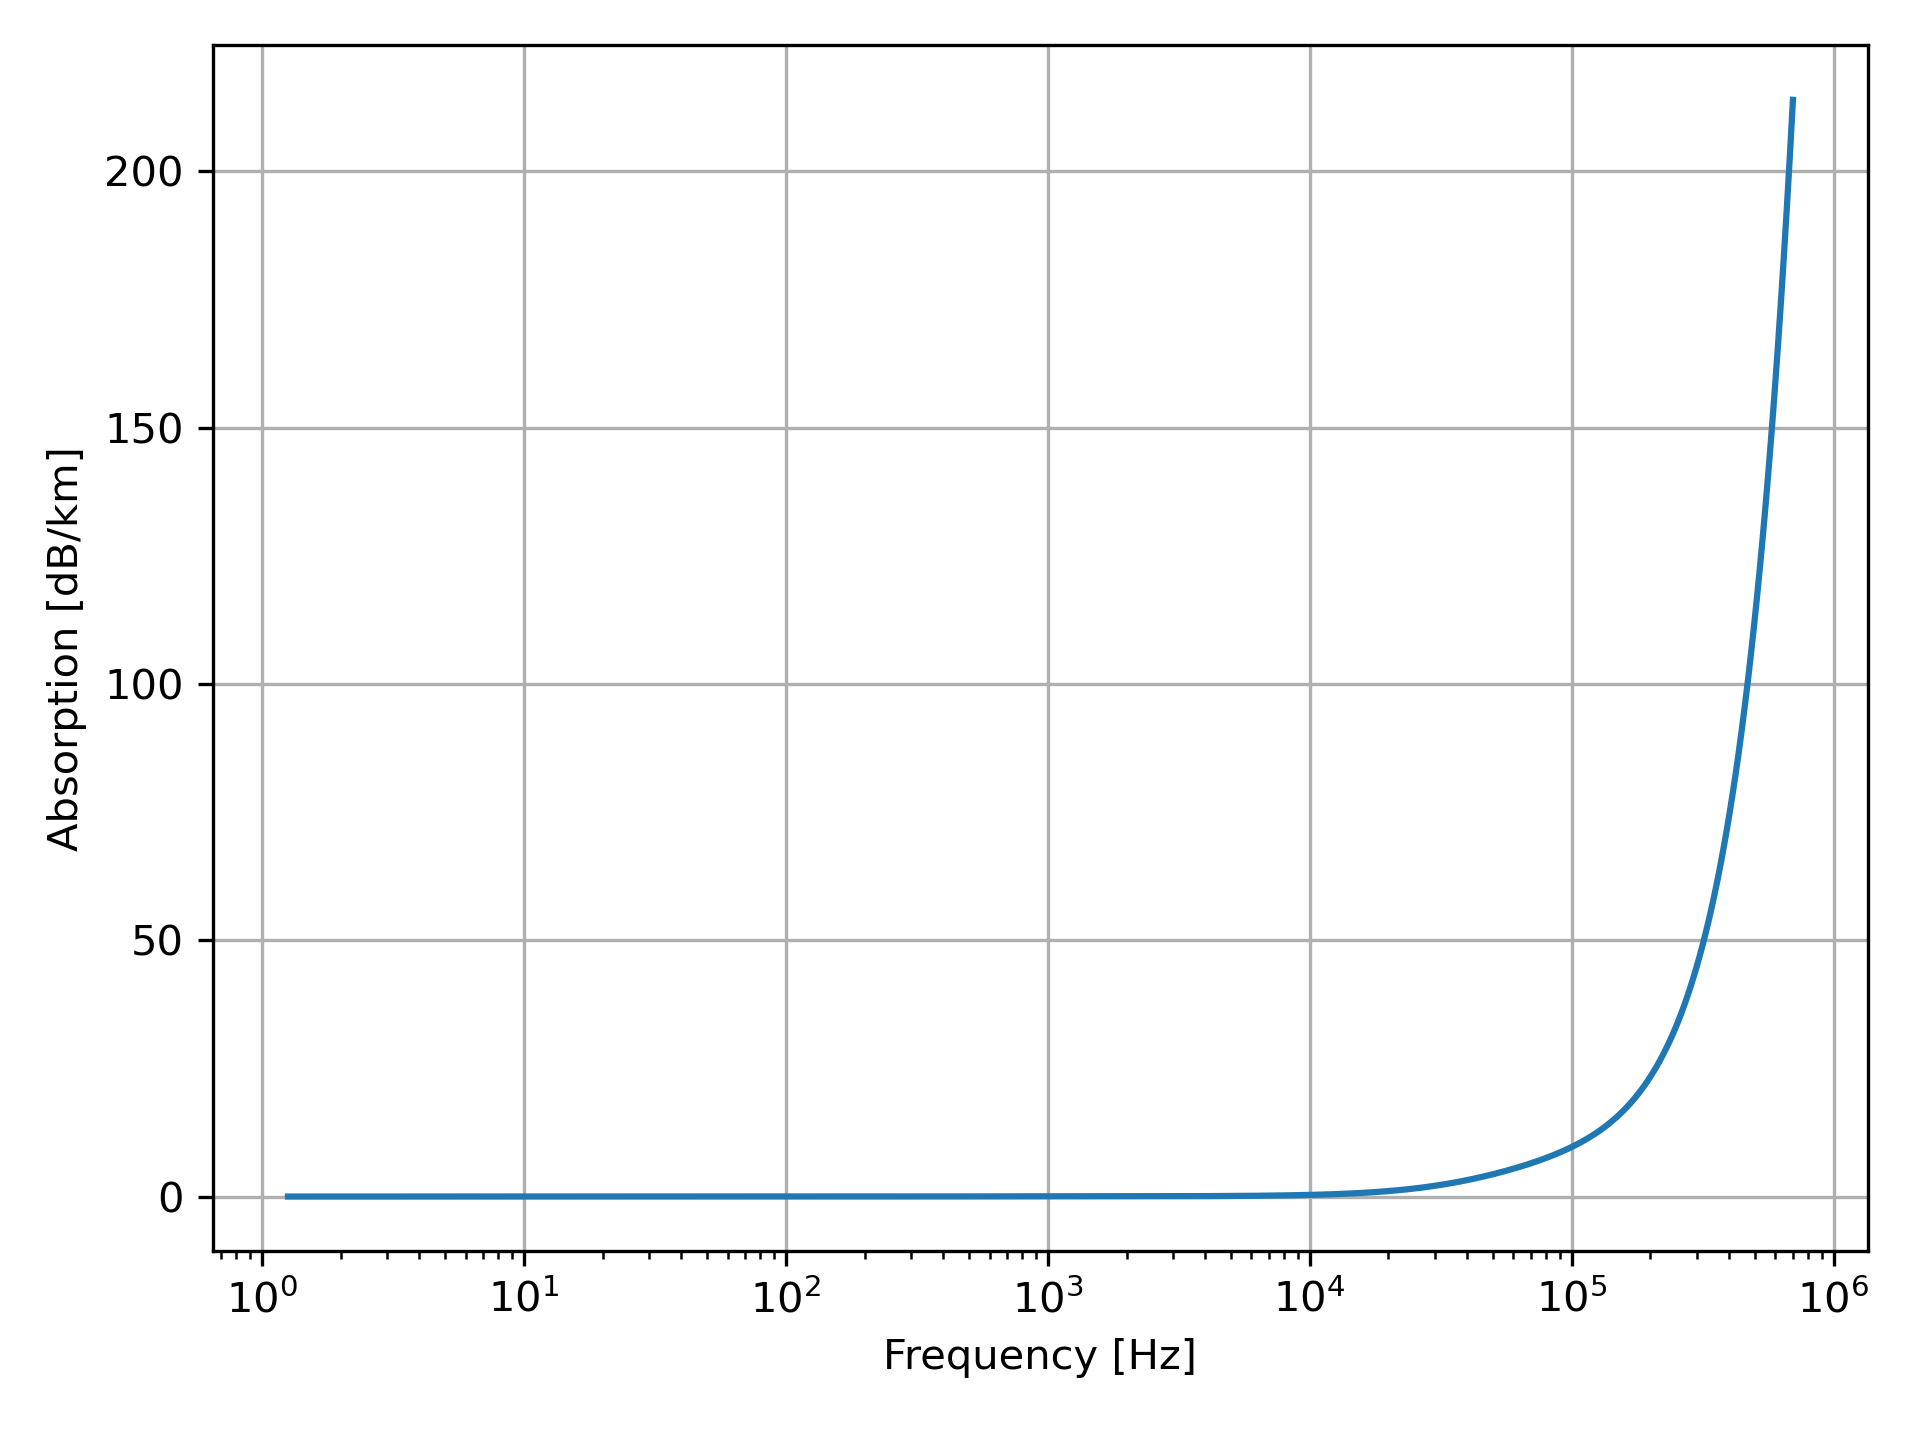
\includegraphics[width=300pt]{Seismics_Absorption}%
\caption{Absorption model.}%
\end{figure}

%
\subsection{Filter Function}%
\label{subsec:FilterFunction}%
The frequency dependent filter function shwon in Figure 4 is calculated                             from the weight function as specified in Southall et al. (2019).%


\begin{figure}[h!]%
\centering%
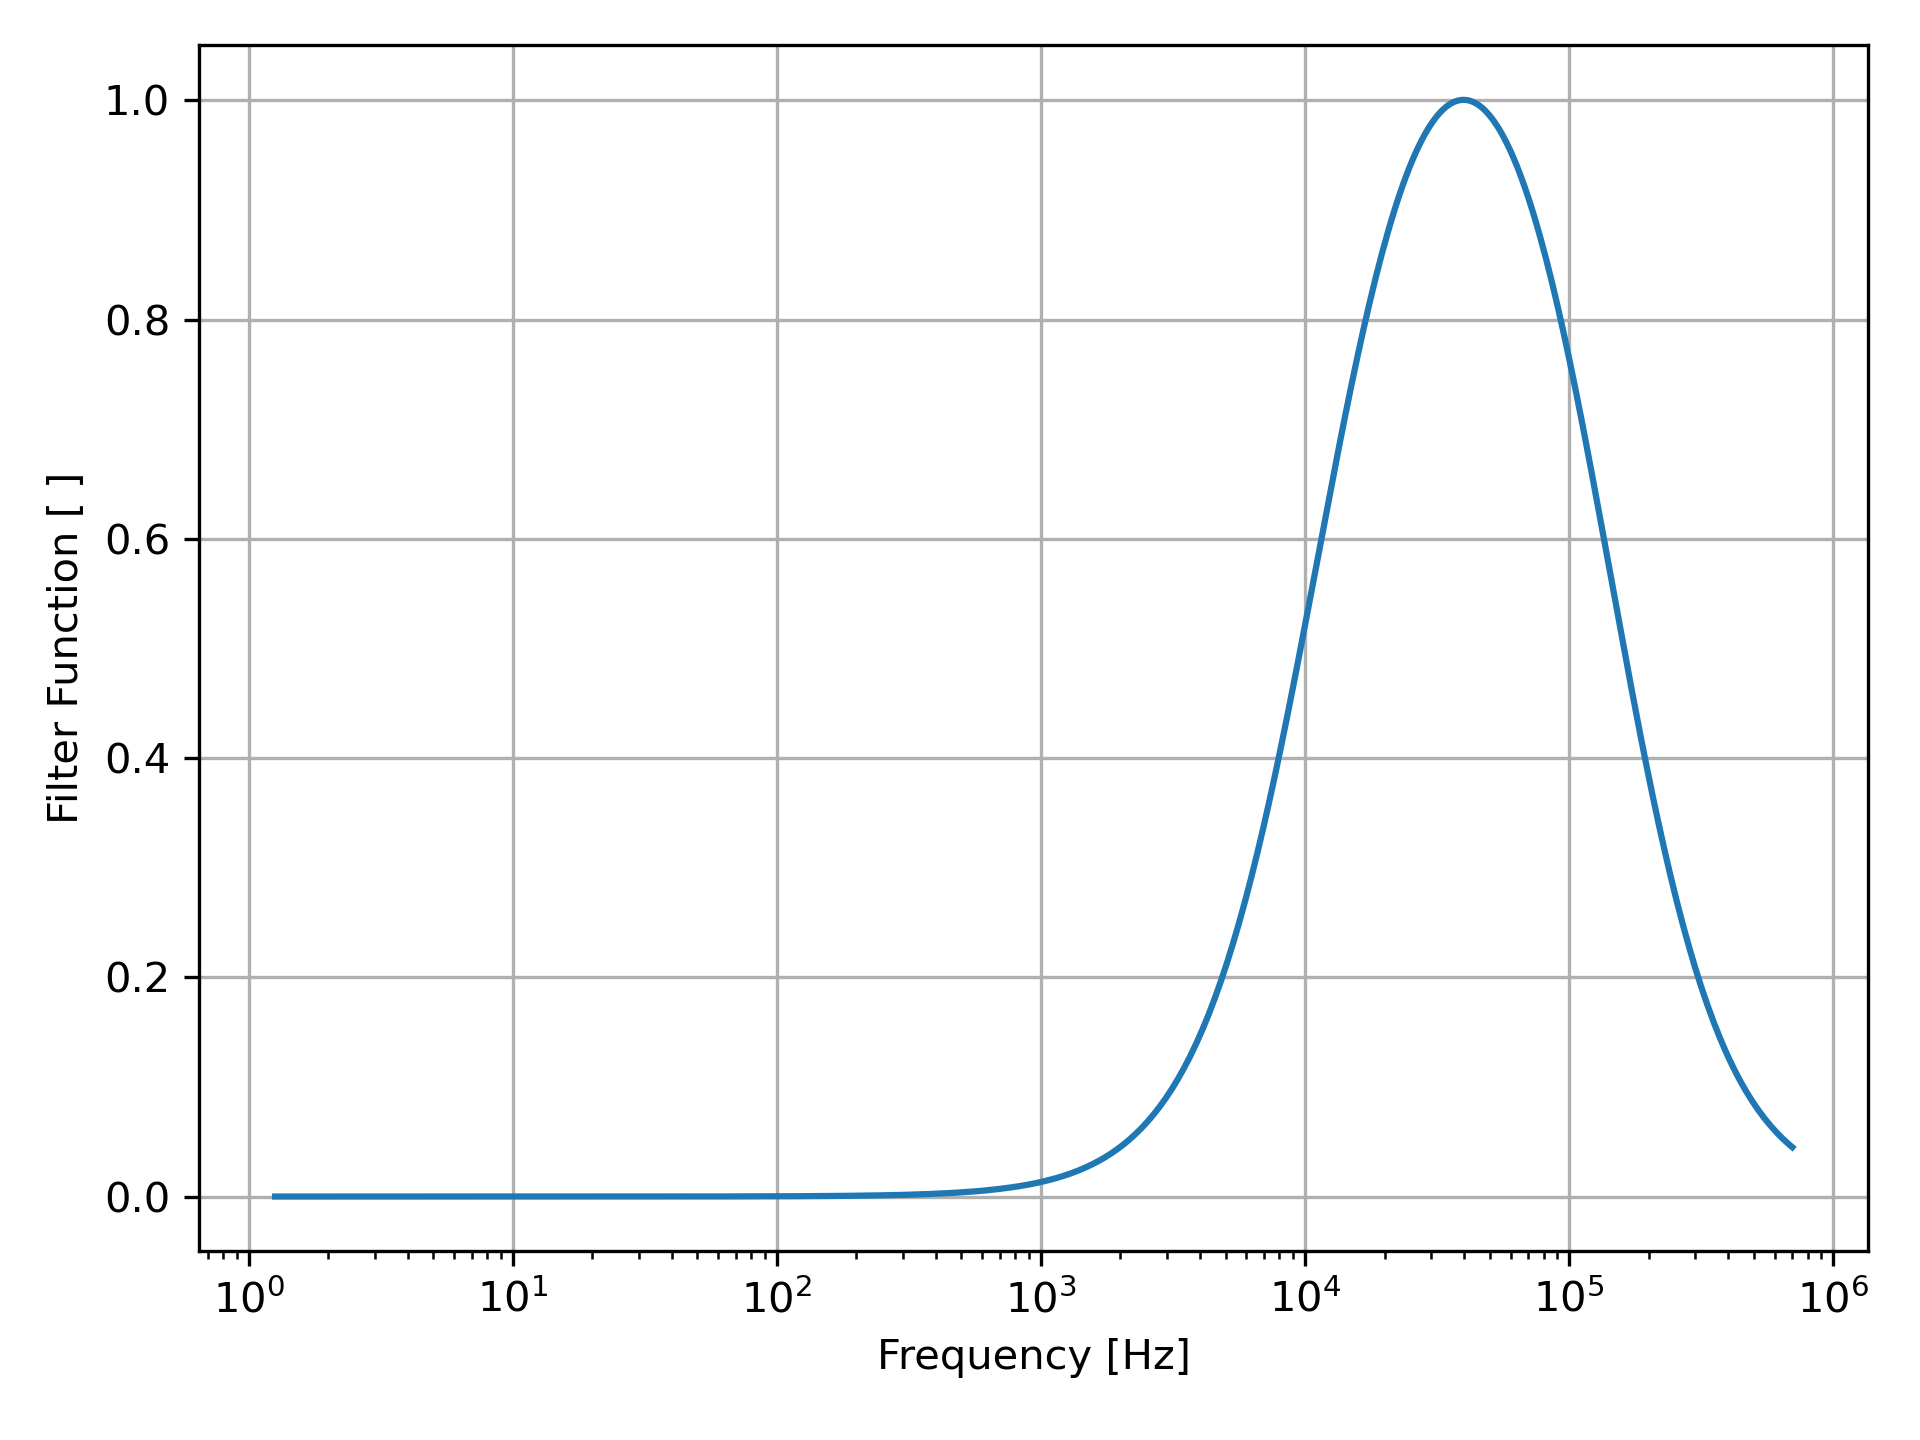
\includegraphics[width=300pt]{Seismics_Filter}%
\caption{Frequency dependent filter function                                             for the functional hearing group VHF.}%
\end{figure}

%
\newpage%
\newpage%
\section{Safety distances}%
\label{sec:Safetydistances}%
The dual exposure metric unweigthed SPL and weighted SEL                     are calculated to determine the safety distances. To give                     conservative distance estimates, the larger distance of the                    dual metric should be considered for both PTS and TTS.%
\subsection{SPL limits PTS and TTS}%
\label{subsec:SPLlimitsPTSandTTS}%
Based on the source signal, absproption and geometrical spreading,                     the PTS onset distance limit is 13.0 m,                     while the TTS onset distance limit is 20.0 m,                     as shown in Figure 5.%


\begin{figure}[h!]%
\centering%
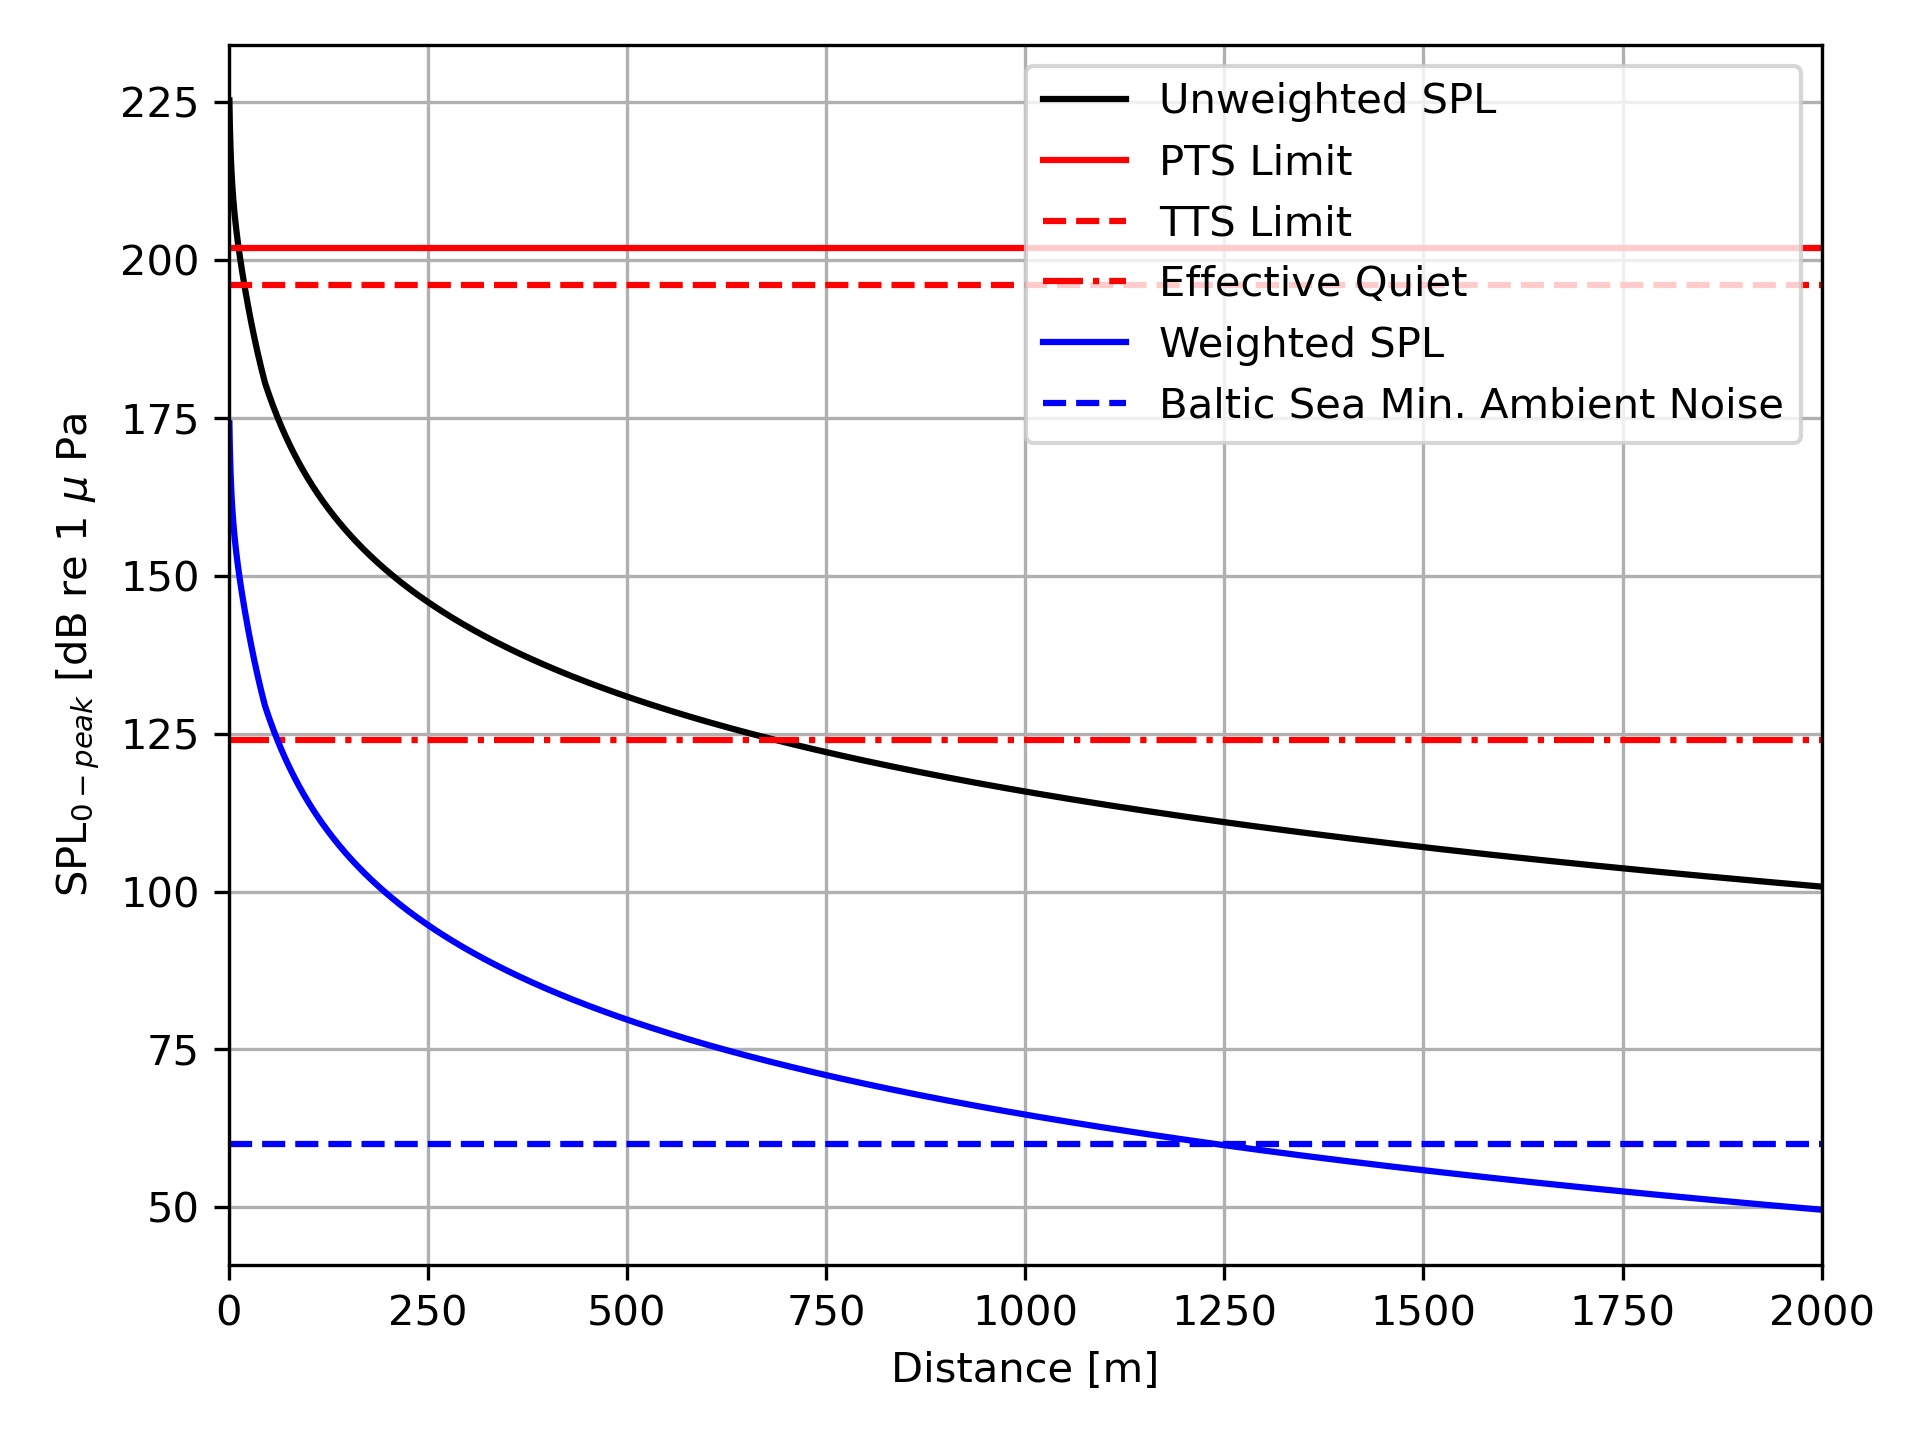
\includegraphics[width=300pt]{Seismics_SPLdist}%
\caption{Reduction of the unweighted zero{-}peak SPL as a function of                     distance to the source with an overlay of the noise limits.}%
\end{figure}

%
\subsection{SEL limits PTS and TTS}%
\label{subsec:SELlimitsPTSandTTS}%
Based on the source signal, absproption and geometrical spreading,                     the PTS onset distance limit is 0.0 m,                     while the TTS onset distance limit is 0.0 m.                    A stationary animal and varying passing distances, which are given on the x{-}                  axis of Figure 6, are considered. For the calculation of the cummulative SEL                  , a profile duration                   of 0.1511 h with a survey speed of 5.0kn and a shot repitition rate of 3.0s are considered.%


\begin{figure}[h!]%
\centering%
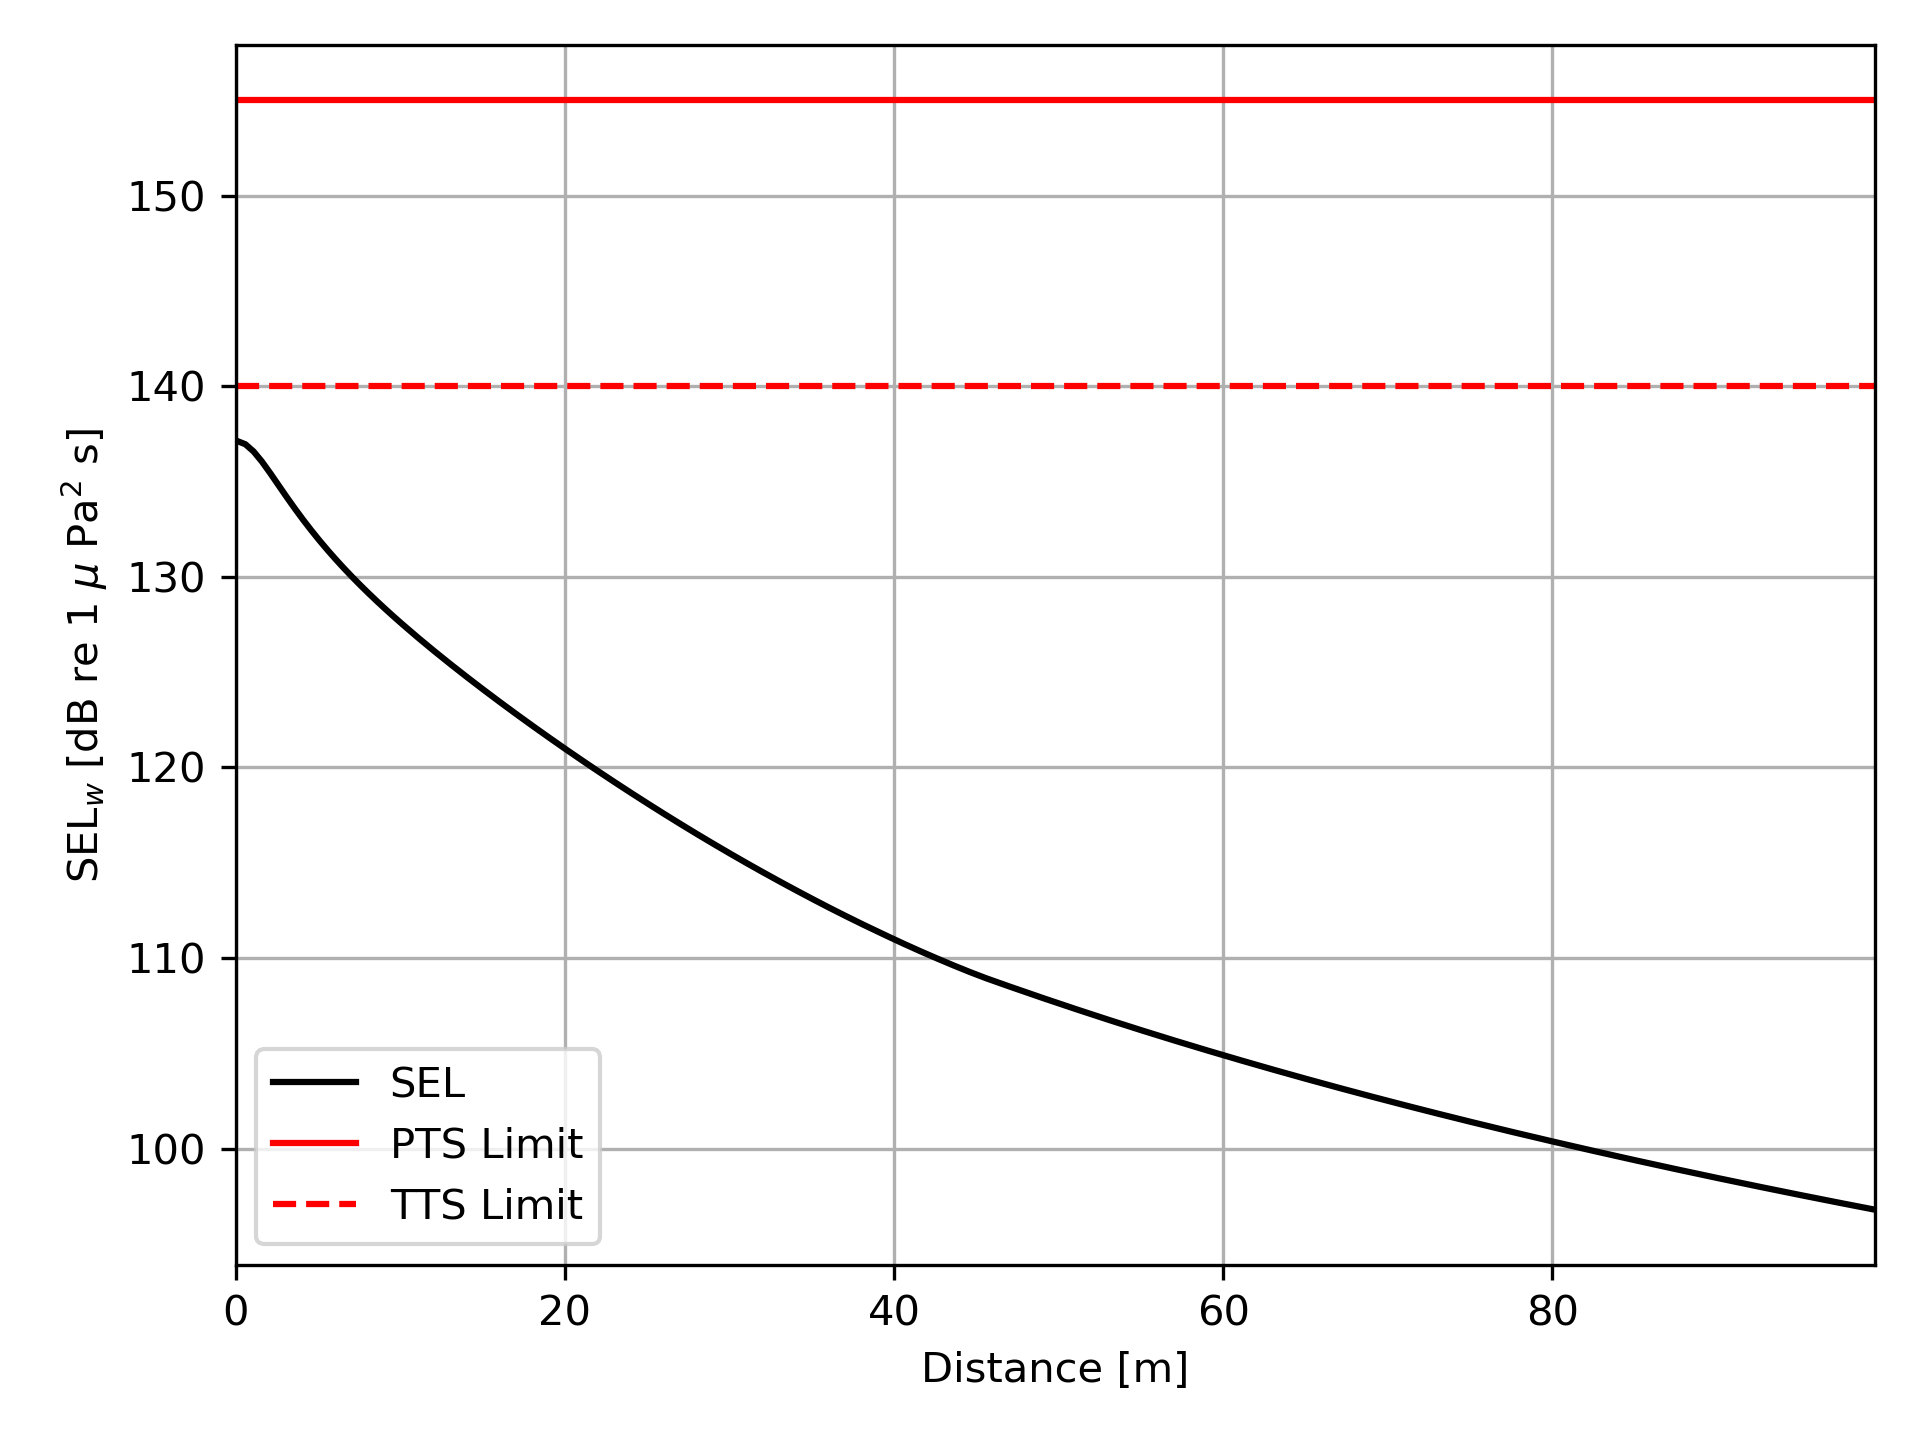
\includegraphics[width=300pt]{Seismics_SELdist}%
\caption{Reduction of the weighted and cummulative SEL                     as a function of the distance to a profile line assuming a                     stationary animal.}%
\end{figure}

%
\subsection{RMS{-}SPL limits Behavioural Impacts}%
\label{subsec:RMS{-}SPLlimitsBehaviouralImpacts}%
Based on the source signal, absproption and geometrical spreading,                     the onset distance limit for behavioural effects is 22.0 m                    as shown in Figure 6.%


\begin{figure}[h!]%
\centering%
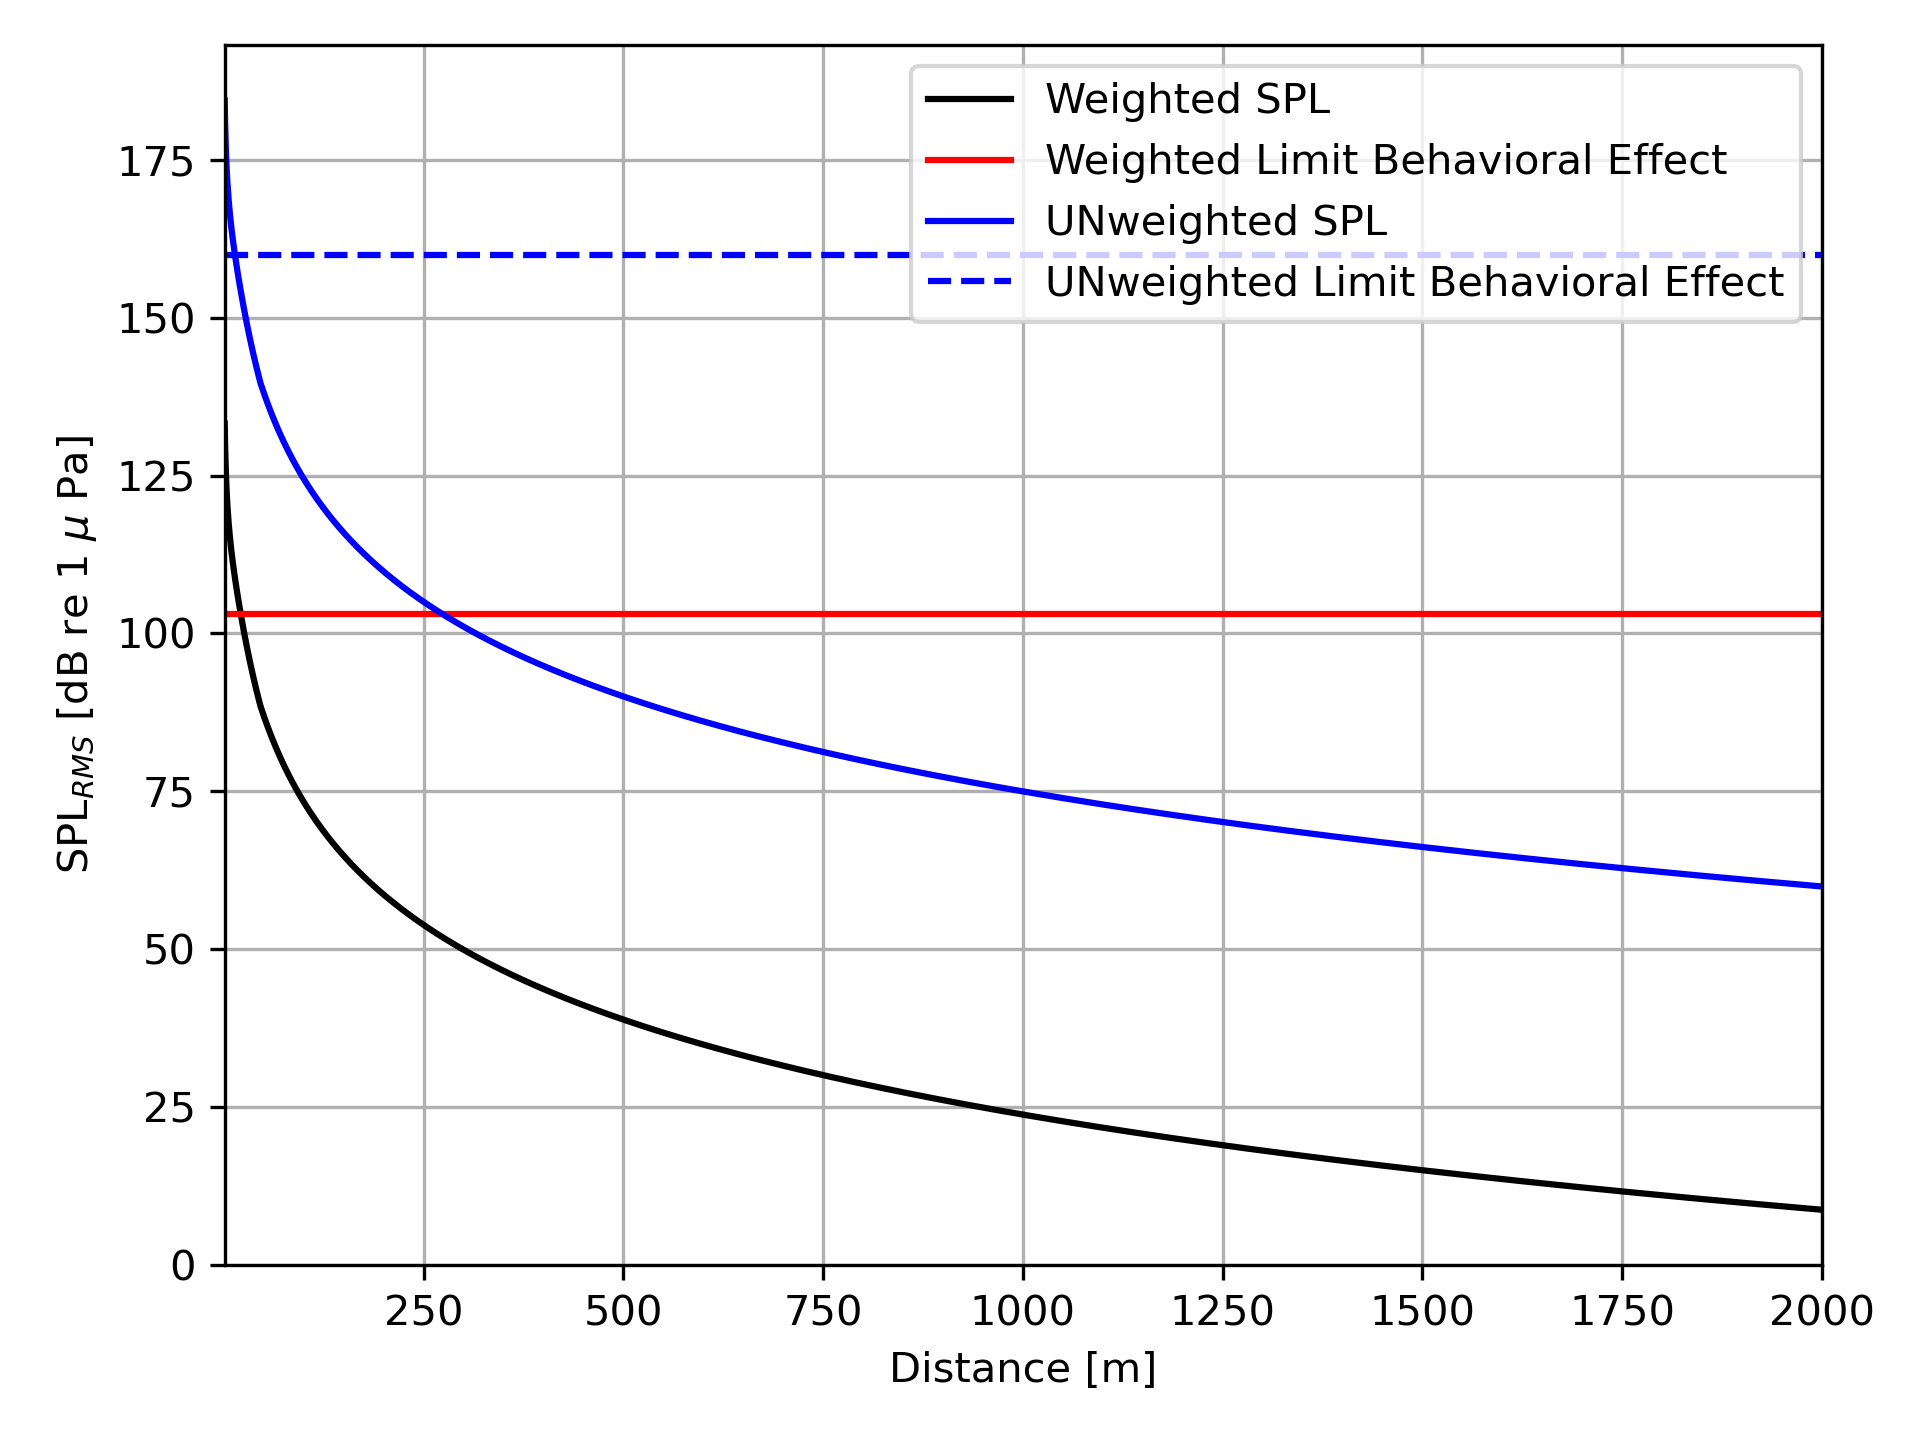
\includegraphics[width=300pt]{Seismics_SplRmsdist}%
\caption{Reduction of the weighted RMS SPL with an                     averaging preiod of 125 ms as a function of                     distance to the source with an overlay of the noise limit.}%
\end{figure}

%
\end{document}